\documentclass{icmmcm}
\usepackage{graphicx}
\usepackage[numbers]{natbib}
\usepackage{url}

\usepackage{csquotes}
\usepackage{titlesec}
\titleformat{\subsubsection}[runin]{\normalfont\bfseries}{\thesubsubsection}{1em}{}
%%% Sample ICM/MCM Contest Submission
%%%
% Copyright (C) 2003-2016  Claire M. Connelly

% This work may be distributed and/or modified under the conditions of
% the LaTeX Project Public License, either version 1.3 of this license
% or (at your option) any later version.

% The latest version of this license is in
%   http://www.latex-project.org/lppl.txt
% and version 1.3 or later is part of all distributions of LaTeX
% version 2005/12/01 or later.

% This work has the LPPL maintenance status `maintained'.

% The Current Maintainer of this work is Claire M. Connelly.



%%% ---------------
%%% Local Command and Environment Definitions

%%% If you have any local command or environment definitions, put them
%%% here or in a separate style file that you load with \usepackage.

% \newtheorem declarations
\newtheorem{Theo1}{Theorem}
\newtheorem{Theo2}{Theorem}[section]
\newtheorem{Lemma}[Theo2]{Lemma}
% Each of the above defines a new theorem environment.
% Multiple theorems can be done in the same environment.
% Theo2's number is defined by the subsection it's in.
% Theo3 uses the same numbering counter and numbering system as
% Theo2 (that's the meaning of [Theo2]).


%%% TeX has an excellent hyphenation algorithm, but sometimes it
%%% gets confused and needs some help.
%%%
%%% For words that only occur once or twice, you can insert hints
%%% directly into your text, as in
%%%
%%%    our data\-base system is one of the most complex ever devised
%%%
%%% For words that you use a lot, and that seem to keep ending up at
%%% the end of a line, however, inserting the hints each time gets to
%%% be a drag.  You can use the \hyphenation command  to globally tell
%%% TeX where to hyphenate words it can't figure out on its own.

\hyphenation{white-space}

%%% End Local Command and Environment Definitions
%%% ---------------


%%% ---------------
%%% Title Block

\title{Pricing Privacy and Personal Information}

%%% Which contest are you taking part in?  (Just one!)

\contest{ICM}

%%% The question you answered.  (Again, just the one.)

\question{F}

%%% Your Contest Team Control Number
\team{87374}


%%% A normal document would specify the author's name (and possibly
%%% their affiliation or other information) in an \author command.
%%% Because the ICM/MCM Contest rules specify that the names of the
%%% team members, their advisor, and their institution should not
%%% appear anywhere in the report, do *not* define an \author command.

%%% Defining the \date command is optional.  If you leave it blank,
%%% your document will include the date that the file is typeset, in
%%% the form  ``Month dd, yyyy''.

% \date{}

%%% End Title Block
%%% ---------------

\begin{document}

% \noindent\includegraphics[height=5cm]{example-image-b.png}

%%% ---------------
%%% Summary

\begin{summary}

% Make the distinction between privacy and PI
We believe that Private Information (PI) and privacy must be clearly distinguished. While PI is just a good that can be traded for benefits between any entities, privacy is the valuable and meaningful personal space that is violated when a third party gets hold of your data.

% first main objective: find an ideal price of privacy and PI
Our first objective is to find an ideal price of PI and privacy. Our main finding here is a generalised model that accounts for both PI and privacy - the PI Equation. It is supported by a Data Valuation Framework, which puts a value on the completeness of the data of an individual and translates qualitative data into a quantity. Together, they help an average person derive the value that he/she should receive in return for a certain amount of data. This enables regulators to set a fair price that data should transact at.

% suggestions of the model
We hypothesize that the difference in prices of PI and privacy is due to market failure, and our model is built based on those assumptions. Eventually, we managed to quantify the factors of imperfect information by grounding our model in reality.

% analysis of model
% strengths and weakness
% sensitivity analysis
Our model gives valuable insight on the differences between PI and privacy and can flexibly account for different companies and individuals, although it is still the most accurate to model transactions between an average individual and an average company. Sensitivity analysis also revealed the effective bounds of the PI Equation.

The PI Equation supports our next objective, which is to come up with a set of policies. PI is a non-rivalrous and easily transferable good, which is why price regulation is difficult to enforce, even if the ideal price is known. The regulation of price is thus not by direct market intervention.

% policies that can drive the current price towards the ideal price, using our model
We suggest three different solutions: strengthening and enforcing existing legislation on data protection, education campaigns to increase the sense of awareness, as well as the promotion and protection of a distributed cryptographic data framework.

Stricter legislation on data protection and higher fines make companies feel the risk of any data breach. Also, the increase of awareness enlightens people on the true price of privacy. Moreover, a robust distributed cryptographic-data framework allows users to benefit from transacting their data without even disclosing it, greatly reducing the risk of selling data.

We then analysed these policies with reference to our model.

% -------------------------------------------------------------------------------------

% We have modelled the individual valuation of personal data. We have confirmed the discrepancy between the valuations of personal data and the individual valuation of privacy. We have some data points to confirm the relationship of the curve. From this we determine what is the fair price. 

% Assumption we take in the building of the model include. (Describe how we handle quality of information.) 

% is ready, individuals, who are not aware of privacy threats, would readily migrate to make use of service that fully respects individual privacy. The impact of these changes are illustrated on our model.

% With our policies we hope our Internet will become one that is both resistant to privacy violations, make use of individuals' data without them giving up their confidentiality.  

%   The contest rules specify that you should include a one-page summary
%   of your report.  This page appears before the rest of the report,
%   and will have a special header attached to it that takes up the top
%   2.5" of the page.

%   By typing your summary inside a \texttt{summary} environment, \TeX\ will
%   handle the formatting of that page correctly, including leaving
%   space at the top of the page and not numbering the page.
  
%   It will also reset the page numbers so that the first page of your
%   report is labelled correctly.
  
%   What should you put here?  Basically, you want a brief restatement
%   of the problem followed by a largely \emph{non-technical}
%   description of what you've done.  Try to avoid using mathematical
%   notation.
  
%   You probably want to write a few paragraphs, around half to
%   two-thirds of a page.

%   In 2016, the COMAP folks said the following:
%   \begin{quotation}
%     The summary is an essential part of your MCM/ICM paper. The
%     judges place considerable weight on the summary, and winning
%     papers are often distinguished from other papers based on the
%     quality of the summary.

%     To write a good summary, imagine that a reader will choose
%     whether to read the body of the paper based on your summary:
%     Your concise presentation in the summary should inspire a
%     reader to learn about the details of your work. Thus, a
%     summary should clearly describe your approach to the problem
%     and, most prominently, your most important conclusions.
%     Summaries that are mere restatements of the contest problem,
%     or are a cut-and-paste boilerplate from the Introduction are
%     generally considered to be weak.

%     Besides the summary sheet as described each paper should
%     contain the following sections:

%     \begin{description}
%     \item[Restatement and Clarification of the Problem] State in
%       your own words what you are going to do.
%     \item[Explain Assumptions and Rationale/Justification]
%       Emphasize the assumptions that bear on the problem. Clearly
%       list all variables used in your model.
%     \item[Include Your Model Design and Justification] for type
%       model used or developed.
%     \item[Describe Model Testing and Sensitivity Analysis],
%       including error analysis, etc.
%     \item[Discuss the Strengths and Weaknesses] of your model or
%       approach.
%   \end{description}
%  \citep{comap-mcm-rules}
% \end{quotation}

\end{summary}
 
%%% End Summary
%%% ---------------

%%% ---------------
%%% Print Title Block, Contents, et al.

\maketitle
\pagenumbering{alph}
\tableofcontents
\newpage
%%% Uncomment the following lines by deleting the % sign
%%% if you have figures or tables in your report:
% \listoffigures
% \listoftables  
 
%%% End Print Title Block, Contents, et al.
%%% ---------------
\section{Introduction}%
\label{sec:introduction}
\pagenumbering{arabic}
\setcounter{page}{1}
\subsection{Should There Even Be a Price on Private Information?}
Before we start evaluating the cost of private information, let us first consider if there should even be a price on private information and what benefits such a price system could provide.

\subsubsection*{Current Situation}
Today, people readily give up their information in exchange for "free" goods and services, for example, by creating an account on a certain platform (and disclosing your private information to do so) to obtain benefits such as electronic books, games, calendar management services or to use a social network platform. Some people even generously fill in their private details on a form just for a chance to win a lucky draw.

The issue with the above situations is that people seem to believe that they have nothing to lose from the exchange as they get "free" goods and services. However, they fail to take into account that their private information has value too. In fact, the value of their private information may be worth more than the few dollars they save from getting the "free" goods and services.

\subsection{Risks of Disclosing Data}
Most individuals today fail to consider the extent at which their data is being used and the risks that they are taking in disclosing their data.
% Furthermore, there are other factors to take into account as well - for example, what the company does to your data afterwards. In spite of all this, most people still assume that entities like data brokers do not have malicious intentions such as doxing and that reputable companies comply with privacy laws and protect consumers’ information. As a result, they usually do not consider the consequences of freely sharing their information in such situations.

\subsubsection*{Unfairness Towards Individuals}
Once companies obtain private information from individuals, these individuals no longer have any control over how the companies handle their data and how securely their private information is stored. There is also a lack of regulations that prevent companies from trading the obtained data amongst themselves to obtain even more benefits. This is especially favourable for larger companies as they have a monopoly over individuals' data and can use it to rake up high profits at their expense.

\subsubsection*{Data Breach}
There are also unexpected risks that arise from sharing your data. Data breaches are increasingly common and have affected large corporations like Uber \citep{uber_breach}, Yahoo \citep{yahoo_breach} and even companies that hold sensitive data like Anthem Inc. \citep{anthem_breach}. After a data breach, individuals' information is compromised and likely to be sold on the dark web, which is accessible to people with malicious intents. Considering the frequency and scale of these recent data breaches and many more that were not mentioned, as well as the personal dangers posed to individuals whose private information has been compromised, it has become necessary for companies to remedy the situation by compensating users in the event of such breaches.

% is the dangerousness of the dark web relevant? 
% is it just a avenue for the transaction of stolen data? 
% \subsubsection*{Hacking and the Dark Web} 
% In addition, there are people with malicious intents who attempt to obtain individuals' data through illegal means, compromising their safety and security. These hackers then sell the obtained data on overlay networks require specific software, configurations or authorisation to access, adding on to the dark web. The dark web is a dangerous place as it is accessed by many cybercriminals who then purchase individuals' private information with malicious intents. Thus, any private information circulated there poses a huge security risk to the unsuspecting owner.
% is there citation here ?

\subsection{Why People Still Disclose Their Data} 
Despite the risks of sharing one's private information, individuals still continue to share their private information freely.  

\subsubsection*{Ignorance}
The main reason for this is that most individuals are unaware of the real dangers of sharing their private information as well as the commercial value that their private information provides to companies. 
% For example, a study (http://www.pewinternet.org/2016/01/14/privacy-and-information-sharing/) done by Pew Research Centre on Privacy and Information Sharing assessed participants on their willingness to trade specific private information for certain benefits. 
Ferenstein Wire \citep{ferenstein_disclose} revealed that common daily scenarios, when phrased differently i.e. explicitly stating the private information extracted in these scenarios, actually resulted in people being less willing to trade in their private information, showing that people did not know the full extent of the private information they were sharing. As a result, individuals do not know how to price their data and often undervalue the actual worth of their data.

\subsubsection*{Convenience and Necessity}
Another reason why individuals readily share their data is due to convenience or necessity. There are times when individuals feel that a particular deal is good enough and do not bother to search for an alternative just to protect their private information, or when a service provided is unique and individuals that require the service have no choice but to comply with the terms and conditions issued. For example, social media sites like Whatsapp and Facebook have become popular sites for companies to communicate with their employees, forcing the employees to share their private information with such sites.
% is there citation here?

% following is from the report
% If you want to have access to the largest, most fantastic marketplace in the world, eBay has to know what you have searched for," Rambam said. "If you want to be able pull a phone out of your pocket and talk on it anytime you want, well, that phone reports where you are 24/7. If it's a smart phone like an iPhone or an Android phone, it tell us where you eat, what books you buy, what restaurants you like."

\subsubsection*{The social benefits of sharing data} 
Individuals share data also because they believe in the welfare generated from learning from their data. Many organisations have built up good reputations and credibility through their corporate social responsibility initiatives.
% There are also other unexpected benefits that arise when people share their data, but these benefits were not taken into account by the people whose data is shared, with or without their knowledge. 
For example, technology companies have been experimenting on tools that benefit the society, such as the early detection of health issues \citep{social_health} and the awareness of suicidal thoughts \citep{social_suicide} and terrorist tendencies \citep{social_terrorist}. Such potential social benefits likely outweigh the occasional privacy concerns of most individuals. 

% recommend delete this section
% Thus, we feel the need to develop a pricing model for data that provides a rough gauge of what we feel is a fair price for different kinds of private information for individuals, companies and regulators. This is to ensure accountability for the data one is responsible for and that individuals and companies are compensated in full during the exchange of data.
% should this be here? it seems like we want to lower the price of PI
% are these points covered somewhere else

\subsection{Commodifying Private Information}
% combine the next two sections
There is no standard to base the price of something as intangible as private information against. It is impossible to come up with a general universal cost for an individual's private information, making it unmarketable.
% Compared to the price of a consumer product like Coke, where the market price is set based on the cost price of producing the Coke, the cost of private information to the individual is in the risks involved in revealing such information rather than the cost of producing it. Consequently, it becomes a question of how much an individual is able to foresee the risks involved and how much the individual values his or her safety. 
% Hence, it is impossible to come up with a general universal cost for an individual’s private information, making it unmarketable.
Moreover, PI is a non-rivalrous and easily transferable good. That is why price regulation is difficult to enforce, even if the ideal price is known.

\subsubsection*{Similarities and Differences Between PI, PP and IP}
Private Property (PP) is easily enforceable as it is easy to build physical barriers to prevent intrusion. An intrusion of PP is highly visible, and intruders are likely liable to condemnation and/or punishments.

Intellectual Property (IP) is less tangible than PP, but still largely enforceable. Despite the rampant pirated media on the Internet, production companies are still able to survive and earn profit through legal means, with the help of piracy controls such as copyright. Moreover, punishments for infringement of IP is stricter on companies to deter the making of monetary profit through illegal means.

However, there is currently no similar protection for Private Information (PI). We have to recognize that once data is disclosed, it is impossible to prevent companies from trading the data among themselves or in any other way beneficial to themselves, especially with the increasing capabilities of technology today.

\subsection{Distinguishing between Private Information and Privacy}
There is also a need to distinguish between \textbf{private information or data} and \textbf{privacy}. People are often willing to exchange their private information for benefits such as discounts and convenience but they are also willing to pay a price to protect their privacy. \citep{OCED}

We believe that the difference lies in the method of valuation - privacy is the valuable and meaningful personal space that is violated when a third party gets hold of your data while private information is a good that can be traded for benefits between any entities, be it individuals or companies.

Generally, people tend to value their privacy, often more than they value their private information. This is evident in the numerous empirical studies conducted to examine the difference between the valuation of personal data and the valuation of privacy \citep{OCED}. We will further emphasise and differentiate between the two in our models.

\section{Assumptions}
\subsection{Scope of Analysis}
The graphs represent an average individual in a single transaction with a single average company.
% what is meant by transaction?
% This shows the aggregated transactions between the individual and the company?
Besides private information, the individual incurs no other costs in the transaction. For instance, the time spent is ignored, or is considered as being absorbed by the Benefit curve (described later). 
% The only cost incurred by the individual is his/her private information.
%  (not very likely users have time for every internet services out there).

\subsection{Quality of Information} 
\subsubsection*{Data Valuation Framework}
Before attempting to arrive at a price for information, we first attempt to quantify the the quality of information transacted, because different amounts and kinds of information are valued extremely differently to different individuals. We make a huge assumption here by coming up with an idea of a totality of all information, where all the information of an individual can be represented by a number, say 1, and that the value of each piece of data is then a fraction of that totality.

Companies value the quality of data based on the amount of economic benefits they can derive from it, be it extra revenue, market share, or customer loyalty. In other words, they value the Private Information objectively as economic goods. We first identified several categories of data \citep{classify_data}. Then, we listed out some of the information that could benefit such companies (refer to Table 1 below).

\begin{center}
\caption{Table 1: The Quality of Information of Personal Data}
\begin{tabular}{ c|c|c }

  &  & Quality of \\ 
 Constituent Factors & Personal Data & Information \\
 \hline  \hline
 Coordinates (0.0006)           & Current Location              & 0.0017  \\ 
 Places Visited (0.0011)        &                               &               \\
 \hline
 Sites Visited/Clicks (0.0024)  & Web Browsing History          & 0.0048  \\
 Time Spent (0.0024)            &                               &               \\
  \hline
 Full Name (0.0028)             & Email                         & 0.0564  \\
 Company Domain (0.0536)        &                               &               \\
  \hline
 Preferences (0.0225)           & Marital Status                & 0.0665  \\
 Spouse Info (0.0440)           &                               &               \\
  \hline
 Medical History (0.0516)       & Health Condition              & 0.1174  \\
 Family History (0.0658)        &                               &               \\
  \hline
 Connections (0.4333)           & Full social network profile   & 0.7533  \\
 Background (0.1202)            &                               &               \\
 Interests (0.1998)             &                               &               \\
\end{tabular}
\end{center}

We are not considering the information sold by hackers, which is a breach of security and not a breach of privacy. We are also not considering the analytic work that data companies might have done to value-add their data product. Here, we are simply considering the value of such raw PI to trustworthy companies and entities.

An average person values the quality of data transacted based on how much meaning or how intrusive the data is to him, i.e. data is valued not based on how useful it is, but how much privacy it infringes upon. We listed out the different types of data (refer to Table 2 below). \citep{data_totalm} 

%% Insert table here

\begin{center}
\caption{Table 2: The Quality of Information of the Privacy Aspects}
\begin{tabular}{ c|c|c } 
 & & Quality of \\ 
 Constituent Factors & Privacy Aspect & Information \\
 \hline \hline
 Gender (0.0021)                            & Gender and Name    & 0.0081  \\
 Name (0.0060)                              &                    &               \\
 \hline
 Spouse Info (0.0172)                       & Marital Status     & 0.0306  \\
 Current Availability / Type (0.0134)       &                    &              \\
 \hline
 People Captured (0.0226)                   & Photos and Videos  & 0.0452  \\
 Places Captured (0.0226)                   &                    &               \\
 \hline
 Household Income Range (0.0504)            & Home Address       & 0.0626  \\
 Household Members (0.0122)                 &                    &               \\
 \hline
 Items Purchased (0.0442)                   & Purchase History   & 0.0781  \\
 Shops/Sites Visited (0.0339)               &                    &               \\
 \hline
 Current Coordinates (0.0926)               & Location           & 0.1170  \\
 Places Visited (0.0244)                    &                    &               \\
 \hline
 Credit Card Number (0.0305)                & Credit Card        & 0.1309  \\
 Expiry Date and CVN Code (0.1004)          &                    &               \\
 \hline
 Date of Birth/Nationality (0.0812)         & ID Number          & 0.1508  \\
 Account User Name (0.0696)                 &                    &               \\
 \hline
 Account Access (0.0956)                    & Passwords          & 0.1832  \\
 Related Passwords (0.0876)                 &                    &               \\
 \hline
 Medical History (0.1934)                   & Medical            & 0.1934  \\
\end{tabular}

\end{center}

% Current location:
% 0.0017
% Web Browsing history
% 0.0048
% Email:
% 0.0564
% Marital Status:
% 0.0665
% Health condition
% 0.1174
% Full social network profile:
% 0.7533

% this one need to be defensible leh

% Privacy

% Gender and name:
% 0.0081
% Marital status:
% 0.0306
% photos and videos:
% 0.0452
% Home address:
% 0.0626
% Purchase history
% 0.0781
% location:
% 0.1170
% credit card:
% 0.1309
% SSN:
% 0.1508
% passwords:
% 0.1832
% medical:
% 0.1934

\noindent
This is how an average composition of information quality might look like. 
As we have no way of finding a universal average of the price of different data types, these values have been obtained by reverse-engineering our model. 
These values will also be used as examples throughout the report.

\section{Base Model}
The central question we are tackling in this model is: \textbf{What should the price of private information and privacy be?} There are three ambiguous terms here - "cost of private information", "cost of privacy" and "should", and all of which must be clearly defined in our base model. 

\subsubsection*{What is meant by \textit{"cost of private information"}?} Since we take "private information" to be the objective economic value of the information, it is simply the price that personal data is traded at between companies. Alternatively, if individuals wish to sell their data voluntarily, it is also considered as the sale of PI and should be judged by this cost as well.

\subsubsection*{What is meant by \textit{"cost of privacy"}?} Since we take "privacy" to be the protection of the individual's personal and meaningful information against unknown entities, the "cost of privacy" is the cost that individuals feel that third parties should pay to access certain information. 

\subsubsection*{What is meant by \textit{"should"}?} It means that the model sets an ideal standard that we should follow, which is a price that is fair to both the data-provider and the data-purchaser. This also begs the question - why are we not already at the ideal?


\subsection{The Initial Idea: the Naive Provider of PI}
The graph here (refer to Figure 1) plots the values of different types of PI per transaction for an average and naive individual.

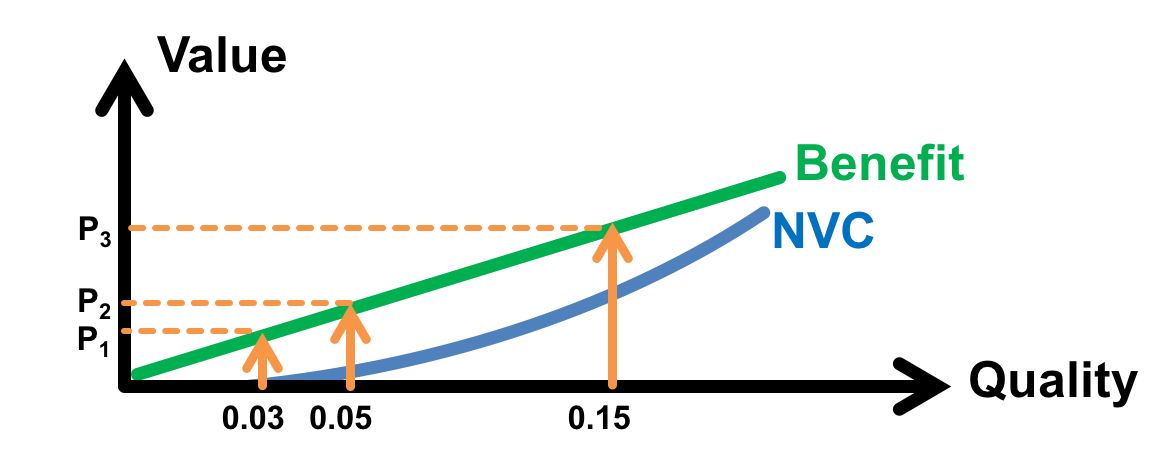
\includegraphics[width=0.75\textwidth]{Picture1.png}
% \rule{.5pt}{5cm} \rule{10cm}{.1pt} \rule{.1pt}{5cm}
\\ \caption{Figure 1: Transaction for an average naive individual}

% Using Facebook as an example. Mark out the points and label them, and use these points.
% (Make the following paragraphs more understandable)
\subsubsection*{Quality of Information} 
The horizontal Quality-axis refers to the completeness of data. The domain of this axis is 0-1, corresponding to the percentage completeness computed using the Data Valuation Framework.

\subsubsection*{Value} 
The vertical Value-axis refers to the value obtained by the data-provider or data-purchaser from a certain transaction. The Value-axis is a generalization of Price to include intangible and non-measurable benefits that applications and services provide. 

\subsubsection*{Naive Valuation Curve} 
The curve in orange is the NVC. Every point on the curve refers to the amount of value naive individuals currently expect when they disclose their information to a trusted company. The naive individuals are unaware of how much their data is really worth, and the true risks involved in providing others with their data.

\subsubsection*{Delta Offers} 
The vertical lines showing the deltas indicate an offer. An example of such an offer could be a \$5 discount voucher if you disclose your payment information. If the payment information is worth 0.2 on the quality scale, this corresponds to a delta offer with a height (value) of \$5 at 0.2 on the quality scale. The delta offers intersect with the NVC at the minimum value at which the naive individual will exchange his or her information.

\subsubsection*{Benefit Curve} Next, we depict a graduated offer system, referring to services which offer increasingly better services with the more information you provide. 
This is similar to aggregating many separate offers (delta peaks) over the 0-1 quality scale. This results in a Benefit curve.

Let us take the use of Facebook as an example. Providing your basic credentials (0.02 quality) gives you access to post your information, shown as benefit $P_1$. Then, you have the option to provide data of your workplace and past schooling experience (extra 0.03 quality) in exchange for the convenience of adding your past colleagues and classmates as friends, shown as benefit $P_2$. Additionally, you can provide your credit card information (extra 0.10 quality) in exchange for gaming services, giving you a total benefit of $P_3$. 

\subsection{The Enlightened Provider of PI}
So how do we find an ideal price for \textbf{privacy} in our model? 
We can borrow the Economics concept of Market failure. We understand that if the individual becomes more informed about 1) the true value of his/her data, and 2) the true risks of sharing data, he/she will request higher prices and value for the PI that he/she provides.

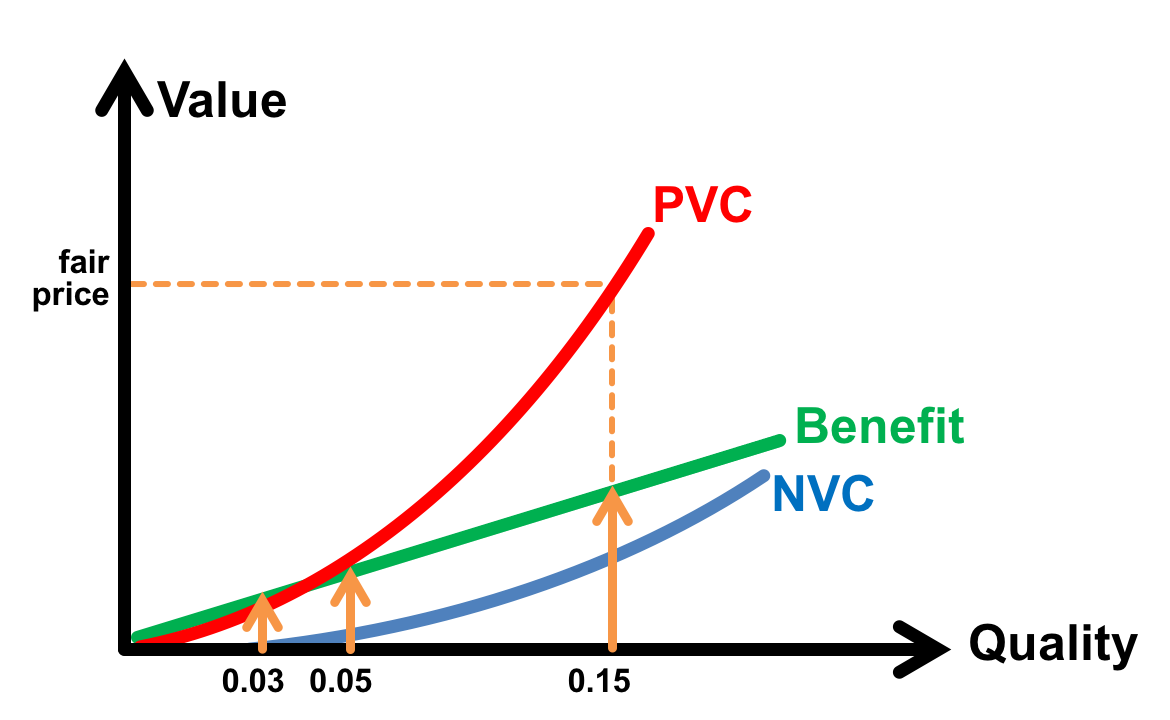
\includegraphics[width=0.75\textwidth, center]{Picture2.png} 
% \rule{.5pt}{5cm} \rule{10cm}{.1pt} \rule{.1pt}{5cm}
\\ \caption{Figure 2: Comparing the Naive and Enlightened Provider of PI}

\subsubsection*{Privacy Valuation Curve} Referring to Figure 2, the PVC represents the true valuations of revealing sensitive personal information by an enlightened individual. We can compare this to the NVC, in which a naive provider is willing to provide his meaningful data for a fraction of the true value. 

\subsubsection*{Ideal Price} The ideal price would then be the intersection between the PVC and the Benefit Curve. This is the fairest price for both the individual who provides the data and the company that buys the data.
% talk about benefit equals cost, best deal ever because no one is worse off?

\subsection{The Risk-Ignoring Companies}

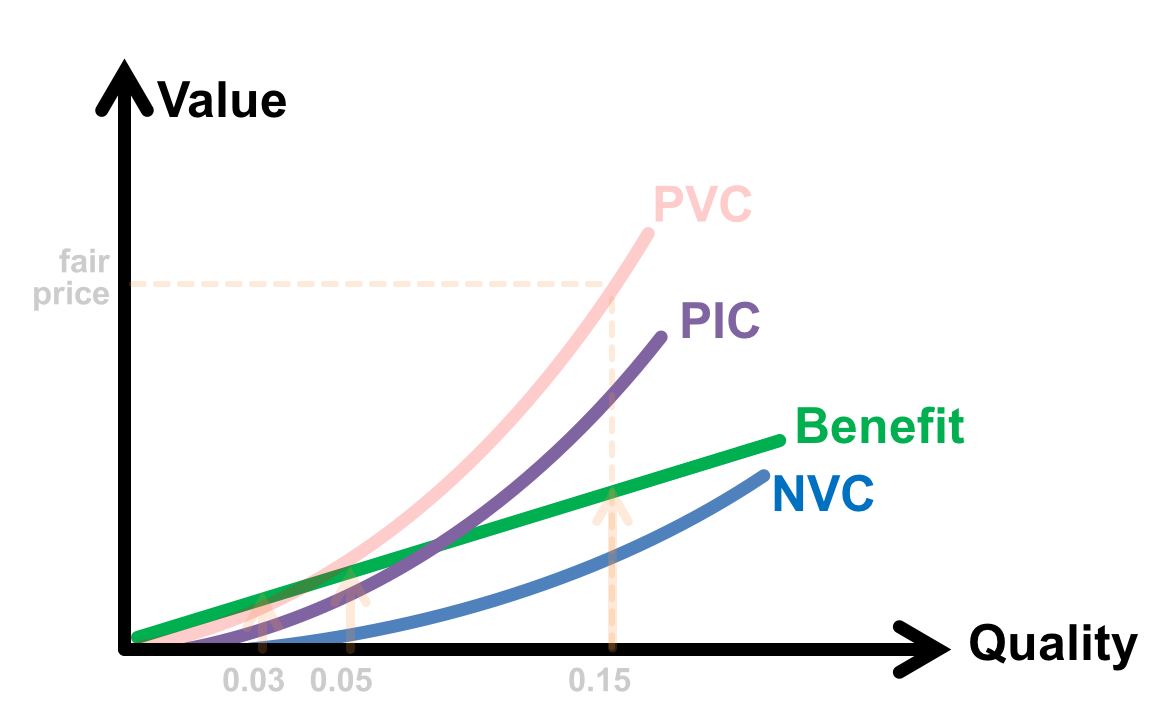
\includegraphics[width=0.75\textwidth]{Picture3.png} \\
\caption{Figure 3: Graph of the Market Valuation of PI} \\

How do we then find an ideal price for \textbf{Private Information}?
Again, we borrow the concept of Market Failure and observe that while companies have close to perfect information of the value of PI, they ignore the risks it brings to the individuals when they sell the information. Thus, they demand a price between the NVC and PVC i.e. the PIC (refer to Figure 3) when they sell the PI to other companies. 

This curve has a grounding in reality and we can find it by searching up the price of transactions of the different kinds of data. 

\subsection{The PI Equation}
$$ V =AB(e^{ln(M) \cdot x^{\frac{1}{b+c}}}-1)$$
This is the equation that models the cost of privacy and PI of individuals, which is a generalization of the PVC, the PIC and the NVC.
\subsubsection*{The Parameters} where:\\
$V$ = value (in dollars) \\
$x$ = data completeness (from 0 - 1) \\
$A$ = risk factor (interpreted as net worth multiplier, which are the losses should the data lead to a security breach) \\
$B$ = discount factor (a \% discount which models the reduction in stinginess of data when it is used for a good cause) \\
$M$ = maximum price (at complete info of 1) which is currently set to 3500 for privacy and 100 for personal data \\
$b$ = level of knowledge of value \\
$c$ = amount of risk considered

\subsubsection{The Exponential Behaviour of the PI Equation}
The equation should be a general model that can compute the value of both PI and privacy. We adopted an exponential form for the equation as we felt that, the more information that people know about us, the more connections and inferences they can make, and the more the sense of violation that we feel. For example, knowing that someone is part of a Facebook group with extreme political viewpoints and that another person is a teacher, is much less intrusive than knowing that the same person is both a teacher and has extreme political viewpoints.

Another way of seeing it is that when people know more pieces of information about us, the amount of information they can infer is not limited to a connection between only those two pieces, but also the connection between all of the pieces of information that they have seen so far. Thus, mathematically, this is not merely a quadratic (finding connection between 2 pieces of information) or cubic relationship (finding connection between 3 pieces of information), but rather an exponential relationship which considers all the subsets of all the information provided.

\subsubsection{The Knowledge Factors Captured in the PI Equation}
The first knowledge factor that we had identified previously was the knowledge of the value of the PI which we denote by a factor $b$. This was the difference between the value demanded by naive data providers (NVC) and the price that companies demanded (PIC) in exchange for data. In other words, $b=0$ or close to $0$ for naive data providers. Our subsequent analysis showed the expected average value for $b$ to be around 0.6811 for a company.

The other knowledge factor that we identified was the knowledge of the risk involved in selling your data, which we denote by a factor $c$. The key difference that we identified between privacy and PI is the awareness of the risks involved. For companies, $c=0$.

The total knowledge factor is $b+c$. The higher the knowledge factor, the steeper the gradient of the curve. % at initial points? the increase is faster?

\subsubsection{The Boundary Conditions of the PI equation}
The PI equation also has 2 important boundaries. Firstly, the value demanded at 0 data should be 0.
Furthermore, the value demanded at quality of data = 1 should be the complete profile of a person. Thus, we include a parameter M which refers to the maximum price demanded for privacy and PI. Mathematically, it is the limit of $V$ as $x$ approaches 1. 
We found that numbers online suggest the price of complete privacy of a person is worth about \$3500. Since companies pay up to \$57 per user profile when they buy a company, our team estimated the cost of a full profile to be objectively worth about \$100. \citep{data_tgd}
% https://thegreatdissonance.wordpress.com/2017/06/03/how-much-is-data-worth/ 

\subsubsection{Consideration of non-average people and non-profit organizations}
After computing the value of the data for an average individual, we added two parameters, A (risk factor) and B (discount factor), to consider for a non-typical transaction. For an average individual in an average transaction, $A=1$ and $B=1$.

The risk factor ($A$) captures the idea that the richer or higher in status one is, the more one stands to lose from disclosing personal information. $A$ can range from 0 (an extremely poor person) to any large number. It can be interpreted as the ratio of the net worth of a person to the net worth of an average individual. This value can also be altered to factor in a person's level of social standing and influence (for example, a country's president might not be very rich but he is very influential).

The discount factor ($B$) considers data transactions that might be used for the common good, such as for security purposes (anti-terrorism). The discount factor can range from 0-1, where 0 means the purpose of the data is so good that it should not be charged, and 1 means that it is for a commercial purpose. 

\subsection{Grounding the Values}
\subsubsection{Obtaining the Data}
The objective value of PI can be represented by the amount of money that companies are willing to pay for each transaction. Here, we mainly used these three sites to obtain data points. \citep{data_ft} \citep{data_totalm} \citep{data_tgd} These sites somewhat corroborate in terms of the value of information and are recent sources of information obtained from companies themselves. Two of them are obtained from the transaction prices of data companies while one is obtained from the selling prices of data-based companies.
% https://ig.ft.com/how-much-is-your-personal-data-worth/ \citep{data_ft}
% http://www.totallymoney.com/personal-data/infographic/ \citep{data_totalm}
% https://thegreatdissonance.wordpress.com/2017/06/03/how-much-is-data-worth/ \citep{data_tgd}

While finding out the value of privacy is much harder, our team based these values on a survey which asked individuals how much they thought their data was worth. This was because individuals' subjective opinions of the cost of their own PI is often more representative of the price of privacy.
Furthermore, the way the company asked the question in this particular survey, "put a cost on a chunk of information that a trusted third party would have to pay to access", suggested the high commercial nature of the transaction, which we think is a good reminder of the value of the PI to companies. \citep{data_trendm}
% https://www.trendmicro.com/vinfo/us/security/news/internet-of-things/how-much-is-your-personal-data-worth-survey-says 


\subsubsection{Comments on Data Collection Methods}
In general, it was hard to find reliable data on how much privacy and PI are worth. Not only were there few studies that provided insights into this issue, the data varied wildly from site to site. Also, the surveys were done on different continents in different years. To standardize, our team always used the most recent data available for a statistic (mostly 2017) and also used data from the US as much as possible. We did not use any data obtained from the prices in the dark web as we feel that those are highly biased values for data that serve different purposes than commercial ones.

Here, we discuss some assumptions that we made, some advantages of our data methods, and some disadvantages.

Using the data from individual surveys might be biased as studies have shown that the values assigned to personal data are highly context-dependent. This means that the results of the survey are extremely sensitive to the phrasing of the questions. There is also a lack of market verification as we cannot check for the validity of these hypothetical prices.
\citep{classify_data}
% http://www.visualcapitalist.com/much-personal-data-worth/

While using the data from companies is good because they are market-verified, they might also not be too accurate because they include the benefits from network effects. They also include the prices of data collection and refinement. \citep{OCED}

\subsubsection{Fitting the numbers}
\label{subsubsec:PVCPIC}
Using the values obtained online (which are organized into a table in the Appendix), we fitted the numbers to the PI equation to obtain the general PIC and PVC (refer to Figure 4).

By rearranging the weights of the Data Valuation Framework appropriately and reasonably, we came up with two equations for an average PVC and PIC, which are:\\
$$ \text{PVC}: V =(e^{ln(3500) \cdot x^{\frac{1}{2.6886}}}-1)$$
$$ \text{PIC}: V =(e^{ln(100) \cdot x^{\frac{1}{0.6811}}}-1)$$

Since $b = 0.6811$, this suggests that an average companies' level of knowledge of the price of information is at about 0.6811.
For an average consumer conscious of his privacy and of the value of his information, $b+c = 2.6886$. 

% (INSERT TABLE IN APPENDIX) convert to graph + cite

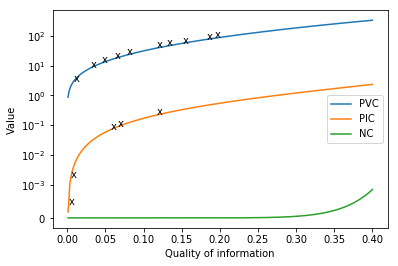
\includegraphics[width=0.75\textwidth]{Picture4.png}
\\ \caption{Figure 4: Our model is based on real price points}

% say that this is linear-log plotted so that we can fit the value on the line haha.
% Insert graph within the value model

\section{Analysis}
\subsection{Strengths}
Our main strength of the model is its ability to differentiate between the value of privacy and PI. The current market prices of PI are simply the companies' transacted values. Thus, we can use the model to determine not only the ideal price for privacy, and also how far away the current prices are from the ideal price. 

Another strength of the model is its illustration of the relationship between the knowledge of the value of PI (b) and perceived risk (c) on the price of PI. This can give us insight on the effectiveness of education and awareness policies.

Our model also finds a way (the Data Valuation Framework) to account for the differing values of different types of information for different individuals. Using the framework, we can also use the perceived values of privacy to find the value of a certain piece of information from the perspective of an individual.

\subsection{Weaknesses}
One weakness of the model is that the model only works best for an average individual and company. This is because many of our approximations were based on the average person/company, which is inevitable as we do not have values or data for special cases, and we cannot really account for it. 

The Data Valuation Framework is highly subjective. In fact, even individuals trying to use the framework for themselves might have a problem quantifying the value of their information. As such, the use of this framework introduces much bias in the model.

The accuracy of our model is also highly dependent on the accuracy of survey results and the veracity of the data we collected. They are also subject to the assumptions we have discussed above. 

Our model also failed to take into account network effects. Data obtained by companies could be worth a lot more just by virtue of being collated in a large number. 

\subsection{Sensitivity Analysis}

\subsubsection*{Sensitivity to the value of an average person's full profile} 
$M$  represents the maximum value. 
% (PLOT GRAPH OF PRIVACY, where M is = 1000, 3500, 5000)
The graph plotted (refer to Figure 5) shows us a family of 3 values: 1000, 3500, 5000.
As the values of $M$ increase, the slopes get steeper and steeper similar to a normal exponential family.

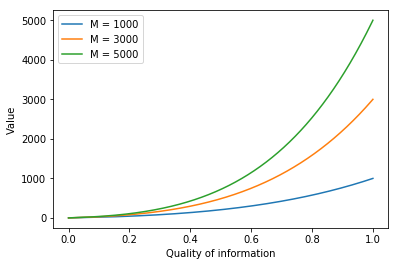
\includegraphics[width=0.8\textwidth]{variousm.png}
\\ \caption{Figure 5: Sensitivity Analysis Graph w.r.t $M$}

\subsubsection*{From the very naive to the very paranoid} 
In general, $b+c$ (information and knowledge of risk) represents the slopes of the curve. The graph plotted (refer to Figure 6) shows us a family of 5 values: 0.001, 2.689, 5.0, 8.16, 14.0.

% (PLOT GRAPH OF PRIVACY, where b+c is = 0.001, 2.689, 5.0, 8.16, 14.0)
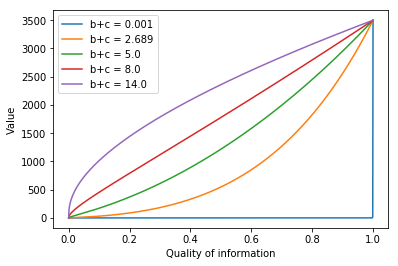
\includegraphics[width=0.8\textwidth]{bplusc.png} 
\\ \caption{Figure 6: Sensitivity Analysis Graph w.r.t. $b+c$} \\

For a very naive person, whose everything else is average but ($b+c$) is close to 0, we observe that the value of privacy is extremely low all the way, until quality of info = 1, where it shoots up to the value of M. The graph looks like an L, which is not realistic as it will probably just be a low value throughout in real life.
As the values increase, the slopes generally get more and more concave.
At the value of around 8.0, the graph becomes approximately linear.
At values of higher than 8.0, the graph becomes logarithmic, which means the model is no longer applicable. 

Hence, our model is only really realistic when b+c is below 8.16, and also shows unintended behaviour at quality of data =1 when $b+c$ is too low.

We also found that this value of 8.16 that we found is dependent on the value of $ln(M)$. We found that the value of a "linear"-looking line, or the breaking point of exponential behaviour, happened when $b+c=M$ approximately.

\subsection{Network Effects of Data}
Other factors external of the individual can also affect the value of the individual’s data. Individuals are part of a network, and when more and more individuals join the same network, network effects come into play, increasing the value and the desirability of each individual’s private information.

While our model currently cannot quantify and take into account network effects, we think that our model has the potential to do so with more data. By observing the changes in $b$ and $M$ that occurs over different network sizes, we can create a separate model that finds the parameters $b$ and $M$ as a function of network size, hence quantifying the network effect.

%One example that shows the significance of network effects is a social network like Facebook. Each time an individual creates a Facebook account and joins the network, the value of the network increases for each existing user, for example through more knowledge being shared, without the intention of the newly joined individual (the individual joined the network for his or her own personal reasons, and not for the purpose of growing the network and giving benefits to existing users).

% citation????

%Similarly, we can apply the network effects to the private information of individuals. As individuals form more networks and connections, for example through meeting new people and making friends, their personal information is highly likely to contain information about other people as well. This makes the individual’s private information much more valuable as attaining the individual’s private information now gives a company clues about the other people in his or her network, from whom companies can then attain their private information. This is with the assumption that groups have similar interests and hence the people in the individual’s network are more likely to be potential consumers for the company as well, allowing the company to benefit greatly from the initial individual’s data. As a result, companies have the incentive to buy data from individuals at a lower cost because after aggregating it, they can derive more value from the data.

\subsubsection{Impact of Network Effects on Our Model and Policy}
Network effects have a significant impact on our model and policy as they heavily influence the value of the individual’s private information. By properly utilizing network effects, the value of an individual’s private information will rise significantly. 

%This is especially beneficial for the individual if he or she knows the true value of his or her private information, and trades it for an equivalent amount of benefits if necessary. As a result, fairness will be enforced as the producer, i.e. the individual with the private information gets compensated for the amount of data revealed while the consumer, i.e. the company receiving the private information, pays the individual with the true value of the data.

\subsection{Applicability In The Real World}
\subsubsection{Comcast case study}
On September 18, 2015, Comcast paid \$100 compensation to each of their 75,000 customers. They were also fined \$33 million. Comcast had published their personal information even though those customers had specifically paid a fee for their information to be kept private - a privacy fee. 
If we calculate the information leaked using our Data Valuation Framework for privacy, including Gender and Name, ID Number and Home address, we get the value of data for an average person to be 0.2215. 
If we use our PVC to find the quality of data that Comcast perceived each customer had lost such that they deserve \$100 compensation, we get the number 0.216. The closeness of these values show the real-life applicability of this model.
% https://techcrunch.com/2015/10/13/whats-the-value-of-your-data/ 
\citep{data_tc}
% https://www.eff.org/deeplinks/2015/10/comcast-agrees-pay-33-million-data-breach-settlement-leaking-thousands-unlisted \citep{comcast_breach}

We feel that this model might also be useful in calculating the compensation for the other massive data breaches, such as Yahoo!'s 3 billion account breach.

\subsection{Future Analysis}
As the saying goes, "data is the new oil." As more and more insights are being developed with data, data is also getting more and more precious and expensive. This effect will be even more obvious, as more and more people are aware of the dangers of sharing their information, as well as the value that companies get out of it.

On the flip side, as more and more data become available, it could also be that the same set of data depreciates over time.

\section{Policies}
As PI is non-rivalrous and an easily transferable good, price regulation is difficult to enforce, even when the ideal price is known. With this in mind, we propose three distinct solutions.

\subsection{Legislation}
In the short term, we should pass pro-privacy laws, and enforce them. 
We should strengthen and execute current privacy laws, like increasing fines, or requiring companies to have robust measures in place to protect individuals' data to minimise chances of data breaches. This legislation will provide the necessary legal foundation to protect individual privacy.

We should also regulate the trading of private information. The intention to sell data should be made explicit to individuals when they contribute their data. We should also enforce that companies allow individuals to download their data any time they want, to allow them to find out exactly what data has been collected from them.

%Moreover, companies are also required to disclose their profit, revenue and expenditure. This will make public the significant potential in the value of individuals' data. 
%Revenue and expenditure records can also highlight companies their possibility of engaging in the trade of personal data.
% We could also consider making the transaction of data across borders illegal. 
% We should also enforce that companies allow individuals to download their data.

% Companies to disclose their profits. 
% Legislate that companies protect users’ data. 
% Use the pricing structure. 
% Make the transaction of data illegal across borders? 
% Transaction of data can still be legal if companies protect individual’s data?
% Enforce the ability for users to download their data. 
% One example is downloading Facebook data.

% Legislate a law that you need to keep data encrypted?

% (Market Equilibrium) The individual want to maximise benefit. They will share information until the difference between the benefit curve and the cost curve is maximised. This is when marginal benefit outweighs the cost. While the individual may want to reveal the juicy details about her past relationship experience for more benefits, perhaps more following, from the platform, she may want to withhold it due because the risk to her is too high. So the individuals would give up that amount of information Q, as such value V.

% (https://www.privacylaws.com/Publications/enews/UK-E-news/Dates/2013/3/ICO-to-evaluate-effectiveness-of-fines/)
% (https://pagefair.com/blog/2017/gdpr_risk_to_the_duopoly)
% (Consider the similar legislation out there already. References needed)

\subsubsection{Illustration On Our Model}
With these laws in place, we believe that companies will at least be cognisant of user privacy in their decision making process. By increasing the fines for a data breach, companies are forced to consider more risks before collecting data, which increases the $c$ for them. The amount of fines for a data breach can be calculated from the model as a function of the $c$ that the regulator hopes to achieve in companies.

We hope that extra risks borne by companies can lead to more stringent measures in processing user data, and avoid the trading of non-explicitly consented personal information to protect their reputation. Moreover, if companies are found to be violating the laws, a punishment can also be extrapolated from the model, which is the total price of all the privacy breached. 

By letting individuals know that their data has been commercialised, and exactly what data has been taken from them, individuals are more informed about the value of their information and the risks that a particular service is putting them through. This increases $b+c$, the awareness of value and risk in individuals. 

\subsubsection{Ineffectiveness of Current Laws}
Despite current laws punishing a mishandling of individuals' data, we still hear data breaches happening from time to time, as mentioned in the introduction.
The root cause is that these companies store data on their servers, which are vulnerable to intrusion. While companies that are more focused on security and privacy like banks would invest more money, firms less focused on security (like Uber) do not have the incentive to make the their data framework fully secure.

We still cannot totally prevent companies from trading the private information without the knowledge of users. However, legislation, while limited in effect, acts as the legal foundation for the individual's right to privacy.

\subsection{Awareness Campaign}
We recommend the decision maker to start information campaigns to publicise the importance of privacy. Though press releases and published information, the decision maker can inform the dangers of disclosing your information. We should also encourage publicity of data breaches to illustrate how real the problem is.

\subsubsection{Illustration On Our Model}
We assume that everyone will have a clearer understanding of the importance of privacy, leading to an increase in $b+c$. We illustrate this by a movement of the NVC towards the PVC (refer to Figure 7). In the example of Facebook, people may no longer want to use Facebook’s messaging function anymore, because those messages might be leaked. If the new PVC no longer intersects the delta function, the user stops using the service.\\
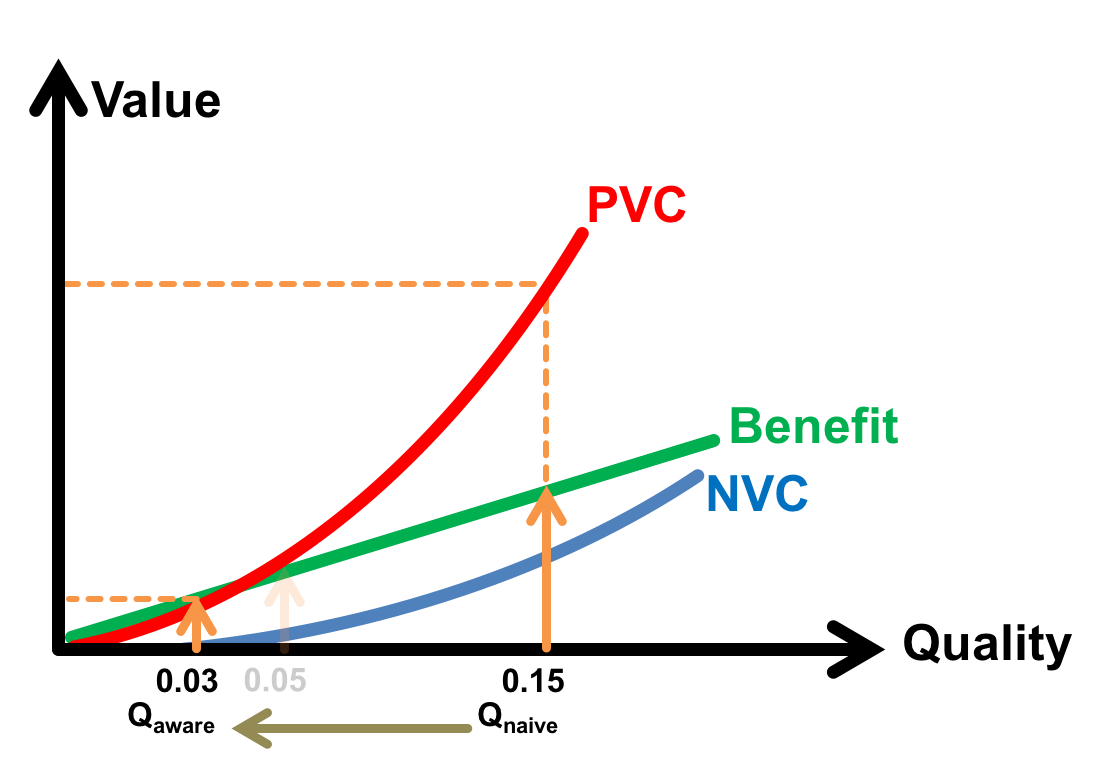
\includegraphics[width=0.8\textwidth]{Picture5.png}
\\ \caption{Figure 7: Effect of increasing awareness on privacy} \\

%Making the entire population paranoid about their data is neither ideal. If all people from now on strongly believe that any information will eventually public, the economy will not function. As the society is made up of communications between one another, that channels that are not fully privacy respecting, society today can longer function without electronic communication.

However, realistically, we will not expect the people to be enlightened immediately. Despite Snowden's highly publicised revelations of NSA's privacy overreach, most of the Americans are still apathetic to the affair. People with high privacy awareness have largely not changed many of their other habits either. One reason could be that alternative technologies such as the Tor web browser are inconsistent and slow. Therefore we need to nurture alternative yet convenient technologies that fully respect the privacy of the users.

\subsection{Restructuring the Internet}
We propose supporting and protecting the development of a decentralised and cryptographically-secure Internet that allows users to participate equally.
% (http://ieeexplore.ieee.org/stamp/stamp.jsp?tp=&arnumber=7163223)
% [CITATIONS!!!]
\subsubsection{Decentralised Cryptographic Data Framework}
\label{subsubsec:decen}
A decentralised cryptographic data framework allows users to sell the benefits from the usage of their data without even disclosing their data. It is possible with a few recently developed methods. There is a group of volunteers currently developing OpenMined \citep{openmined}, a distributed data framework with deep learning, federated learning, homomorphic encryption as well as blockchain smart contracts. It assumes a fully rigorous framework and a trusted and verified third party known as the Oracle. A more in-depth description of this framework can be found in the Appendix.

\subsubsection{Capabilities of a Crypto-Data Framework}
Users can now allow their private data, such as their chat or search history, to be used for training a model without divulging the data at all. The user can also be compensated fairly every time the data is being used. Similarly, companies can utilise people’s data without ever knowing or accessing the data. 
% This is a step to fulfilling the original dream of the Internet to be decentralised and equal.
\subsubsection{Effect of the Crypto-Data Framework on our Model}
As people are guaranteed that their data will not be shared, more people are willing to share the benefits of their data at a low price. In other words, the value of $c$ decreases sharply, even close to 0. This will decrease the PVC curve to low levels close to the PIC (refer to Figure 8) and allow companies to utilise data for cheaper prices. We think that this is the win-win situation that allows users to benefit from their data without risk, and for companies to use data without spending a fortune.

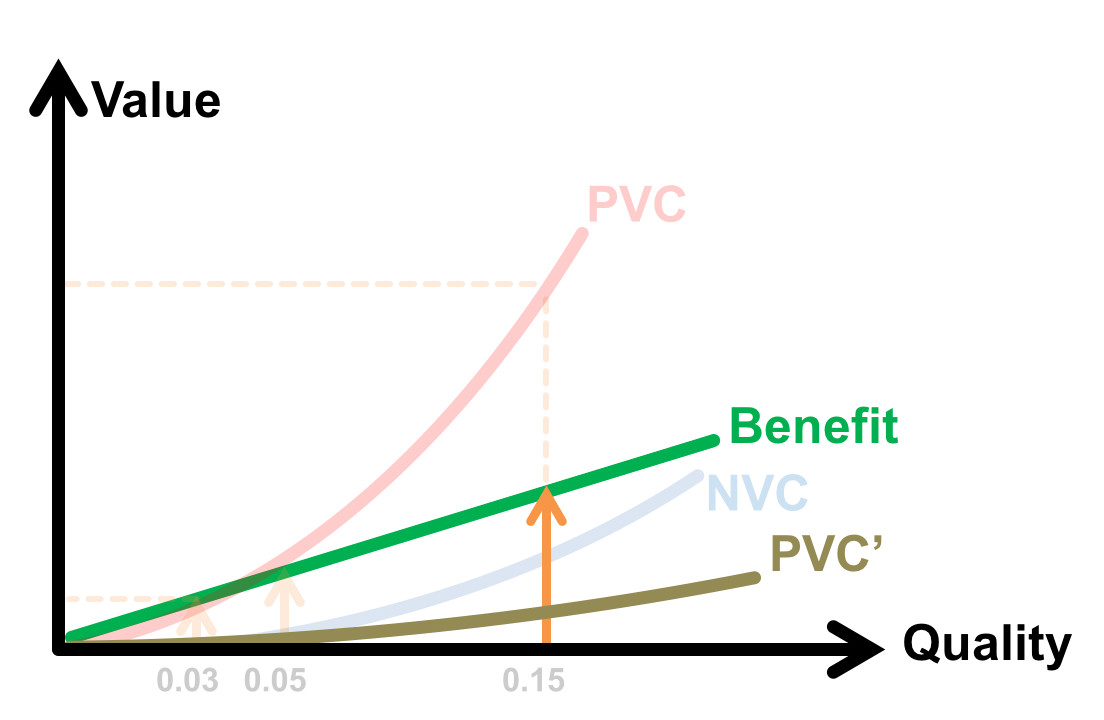
\includegraphics[width=0.8\textwidth, center]{Picture6.png}
\\ \caption{Figure 8: Effect of the Crypto-Data Framework} \\

We foresee that people "paranoid" about their own data will be the first adopters of such decentralised services. As more people realise the benefit of not having their data stolen, they will also move on the decentralised data framework.

%Individuals do at least have a want for privacy, if asked. In recent years we have seen the rise of apps that market themselves with privacy features, such as Telegram and Snapchat. While these apps may not be rigorously secure \citep{telegram}, it illustrates the current desire for access to privacy of many people. Moreover, the society can make use of the vast amount of data to provide more value to the economy, and also for altruistic purposes. 

\subsubsection{Limitations of developing the Crypto-Data Framework}
While the decentralised artificial intelligence framework is in development, the state-of-the-art cryptographic algorithms were still the same ones we used since the start of the millennium. \citep{NIST} The important question to consider: why there is such a lack of privacy-focused services in the first place? This could be mainly attributed to the lack of awareness of data privacy from individuals, which we hope will improve over time through our education campaigns.

Moreover, it is difficult to start a decentralised application given the pervasiveness of the major players in the tech market. Diaspora \citep{disapora} is proposed to be a decentralised social media framework, but its size pales in comparison to Facebook, and the benefits of privacy are insufficient to convince the users to move away from the comfort and wide network on major social networks. There is no competing alternative version of the platform that is decentralised and focuses on privacy.

\subsubsection{Support Required}
Therefore we call for the support the growth of decentralised frameworks so that the user has full control over their data and can benefit from any use of their data. It is best that we start supporting and protecting the decentralisation of the Internet for the good of the people and companies.

\section{Conclusion}
In summary, we have quantified personal information in terms of normalised quality of information using the Data Valuation Framework. We then used the quantities to provide a pricing structure for PI and privacy. Using the pricing model, we then recommended the policies of stricter legislation of data, greater awareness, and the wider adoption of a decentralised cryptographic data framework.

\newpage
\section{Policy Memo}
Dear Decision Maker %(I don’t think we will be showing any graphs here)

In the age of big data, where "data is the new oil", we feel the need to re-emphasise the status of privacy as an inherent human right. Private information (PI) is being sold by the millions at data companies while the individuals themselves, whose data is being sold, are given barely any benefits. Yet individuals are the ones at risk when data breaches occur. PI such as addresses, phone numbers, medical information, marital status and so on can seem trivial to the some, but it can mean a lot to some others.

We hypothesise a few reasons for this problem: people do not know the real value and risk of sharing their PI, and companies also do not care about the risks they bring to individuals when their data gets sold. In other words, market failure due to imperfect information and inequitable risk.

It is also not simple to develop a policy for re-pricing of PI and privacy for two reasons. Firstly, PI and privacy are clearly different things - while PI is just a good with an objective value that can be traded for benefits, privacy is the valuable and meaningful personal space that is violated when a third party gets hold of your data. Differentiating between the prices of the two is already a difficult task.
Secondly, PI is also  a non-rivalrous and easily transferable good, which is why price regulation is difficult to enforce even if the ideal price is known. The usual methods of direct market intervention and taxes are thus unfeasible methods of price regulation. 

In order to support strategies, we first present our method to find a fair price for PI and privacy.\\

Our method is centred around two main models: the Data Valuation Framework, and the PI Equation. The Data Valuation Framework is a method to transform some types of data into a value between 0-1, with 1 being the complete profile and information of a person. Thus, the Data Valuation Framework provides a numerical value on the quality of certain types of information. After calculating a quality-value, it is then utilised in the PI Equation.

The PI Equation is specifically built contextually on the hypotheses of our problem - that market failure is caused by imperfect information and inequitable risk. By assuming the exponential nature of the information curve and setting certain boundary conditions, we managed to ground our model in reality using data obtained from a few recent studies. We realised that  our  model  gives  valuable insight  on  the  differences  between  PI  and privacy. As our model focuses on a transaction between an average individual and average company, it is also suitable for use at any scale - be it groups, companies and entire nations - as long as the knowledge and risk parameters of the entity have been empirically determined.

Comparing the data from our models to the Comcast data breach in 2015, we managed to obtain values of privacy very similar to the valuation by the authorities. This shows that our model has true practical value. \\


Now that we can have a quantity for the ideal price of PI and privacy, we offer our solutions to this problem.

1) Legislation. In the short term, we propose passing pro-privacy laws such as increasing the fines for a data breach, and enforcing regulations to be more transparent about commercialisation of PI.

We propose that fines can be calculated using the cost of privacy calculated in our model. The effectiveness of enforcing transparent commercial interests using the data can also be quantified and measured in our model.

2) Awareness Campaign. We propose starting an information campaigns to publicise the importance of privacy. Again, the effectiveness of the campaign can be quantified and measured in our model, which can help by being an indicator of progress.

3) Restructuring the Internet. We propose supporting and protecting the development of a decentralised and cryptographically-secure Internet that allows companies to utilize users' data in their analysis without accessing or viewing the users' PI. 

We propose that the use of a decentralised cryptographic data framework can help both the individuals and the companies by reducing the risks of sharing data to nearly zero. This is phenomenon is also captured in our model. In such a way, individuals can trade their own PI without the risks, and can thus objectively treat it as a good.

We are in the midst of what is termed as "the fourth revolution" - Artificial Intelligence - that development is fuelled heavily by data. As time passes, data will only become more and more sought after and valuable. We beseech you to consider our proposal to solve the problem and implement them as soon as possible. \\

\noindent
Regards \\
Team 87374
\newpage

%% Outline of memo

%% Describe the problem
% what is the problem
% The current problem that we are attempting to tackle is that people do not know the real value and risk of sharing their private information
% stakeholders
%We are only looking at the PI and privacy of individuals, rather than including companies and nations because individuals are affected the most from the problem mentioned above.
% risks to stakeholders
% emphasise importance of problem
%It is vital to solve this problem as quickly and as efficiently as possible as privacy cannot be replaced once lost. Hence, the problem should be prevented before it spirals out of control.

%% Hypothesised macro-strategy (reduce externalities / information gaps / risks / naivety)
% root of problem
%although it is still the most accurate to model transactions between an aver-age individual and company. Sensitivity analysis also revealed the effective bounds of the PI Equation.
%---------------------------------------------------------------
%Strategies and Policy Modelling
% - policy (related to macro strategy)
%     - what are the policies?
%     - why these policies?
% - model to quantify cost of policies (how much to change by)
%     - explain what the model is
%   - explain the strengths and benefits of the model (utility)

% Results and Recommendations
% - briefly explain some numerical results
% - types of PI
% - develop some recommendations based on results


% % -------------------------------------------------------------------------------------

% (Introduction to privacy) Privacy is an inherent human right and a requirement for maintaining the human condition with dignity and respect. There should be a price to privacy. Citizens' privacy is a national issue. Entities can interfere with our national decisions by targeting the masses with customised misinformation campaigns. 

% % Make the distinction between privacy and PI
% We believe that Private Information (PI) and privacy must be clearly distinguished. While PI is just a good that can be traded for benefits between any entities, privacy is the valuable and meaningful personal space that is violated when a third party gets hold of your data. 
% % Individuals value this different and that is an issue?


% % first main objective: find an ideal price of privacy and PI
% Our main contribution towards the first objective, which is to find an ideal price of PI and privacy, is a generalised model that accounts for both PI and privacy, the PI Equation. It is supported by a Data Valuation Framework, which puts a value on the completeness of the data of an individual and translates qualitative data into a quantity. Together, they help an average person to derive the value that he or she should receive in return for a certain amount of data. This enables regulators to set a fair price that data should transact at.

% % suggestions of the model
% We hypothesise that the difference in prices of PI and privacy is due to market failure, which is captured in our model. A successful feature of the model is that we managed to quantify the forces of imperfect information through grounding our model in reality.

% The PI equation supports the next objective, which is to come up with a set of policies. PI is non-rivalrous and an easily transferable good. That is why price regulation is difficult to enforce, even when the ideal price is known. To circumvent this, we propose three different solutions.

% (Individuals value privacy differently from private information) Research after research has shown that individuals tend to mis-value their privacy and private information, in fact, this holds more true for privacy than their private information. While individuals are willing to exchange some of their personal information for certain benefits, they are willing to pay much more to perfectly reverse a data breach i.e. completely cover up their private information after it has been revealed.

% (Our model) The normalised quantity of information. We have illustrated the discrepancy with the two curves. While the individual may be comfortable in giving pieces of information to trusted sources at a low value, they are vigilant against, and the rapidly increasing curve illustrates the relationship. The bottom curve refers to the individual valuation of their own personal information, while the top curve refers the individual valuation of their privacy.

% (The resulting market failure due to imperfect information - explain only)

% (The resulting market failure due to inequity - companies monopolising data?)

% (Analysis of our model)

% (Network effects)

% \subsection*{Policy}
% As PI is non-rivalrous and an easily transferable good, price regulation is difficult to enforce, even when the ideal price is known. Therefore we propose three distinct solutions.

% \subsubsection*{Legislation}
% In the short term, we should pass pro-privacy laws, and enforce them. We should strengthen and execute current privacy laws, like requiring companies to have robust measures in place to protect individuals’ data to minimise chances to data breach. Legislation provides the necessary legal foundation for to protect individual privacy.
% % Despite of current laws punishing a mishandling of individuals’ data, we hear data breaches happening from time to time, as mentioned in the introduction. 

% \subsubsection*{Awareness Campaign}
% We recommend the decision maker to publicise the importance of privacy and begin an information campaign. We need to let the people know, though press release and published information, on the dangers of disclosing your information to the public. We should also encourage publicity of data breaches to illustrate how real the problem is.

% However, inculcating privacy awareness takes time. Moreover, privacy-savvy individuals has a lack of alternatives to migrate it.

% \subsubsection*{Restructuring the Internet}
% A decentralised cryptographic data framework allows users to sell the benefits from the usage of their data without even disclosing their data.
% It is possible with a few recently developed technologies like federated learning and blockchain. 

% Given the pervasiveness of the major players in the market, it is difficult for a decentralised alternative to gain market share. This requires the majority of the individuals to focus on privacy, as also laws that uphold and protect privacy.

% conclusion?
% Therefore we call for the support the growth of decentralised frameworks that that only the user full control over their data. It is best that we start supporting and protecting decentralisation of the Internet for the better of the people.

% % one page of policies
% (Policies - legislation) We need to strengthen our data protection.
% However, the end goal is not to let companies get in the way monopolising data control.

% (Policies - awareness)

% (Policies - crypto-data framework)

% The original dream for the web, was for everyone to participate in the common neural equally for the betterment of the humanity. The web first pioneers had the ethos that data should be freely available for all that wanted. However, we are far from the goal. 

% Briefly explain what is it and its potential benefits, and the state the issue why this is not implemented.

% We look forward to your resolute decision to protect citizen privacy. Please fund and protect decentralisation of the Internet for the better of the people.\\

% % analysis of model
% % strengths and weakness
% ...
% % sensitivity analysis
% ...

% % policies that can drive the current price towards the ideal price, using our model
% We suggest three different solutions: strengthening and enforcing existing legislation on data protection, education campaigns increase the sense of awareness, as well as the promotion and protection of a distributed cryptographic data framework.

% Legislation on data protection internalises the risk to the companies (makes the companies feel the risk of the data breach). The increase of awareness enlightens people on the true price of privacy, and a robust distributed cryptographic-data framework allows users to benefit from transacting their data without even disclosing it.

% We then analysed these policies with reference to our model.

% Regards \\
% Team 87374
% \newpage

\section{Appendix}
\subsection{PVC and PIC data points}
For the graph in section \ref{subsubsec:PVCPIC}

\begin{center}
\begin{tabular}{ c|c|c } 
 Privacy Aspect & Quality of Information & Value \\ 
 \hline  \hline
 Gender and name          & 0.008102356              & 2.9  \\ 
 Marital status  & 0.030562818          & 8.3  \\
 photos and videos             & 0.045238707                         & 12.2  \\
 Home address          & 0.062646252                & 17.4  \\
 Purchase history       & 0.078099395              & 22.6  \\
 location          & 0.116972815   & 38.4  \\
 credit card          & 0.130906643   & 45.1  \\
 SSN          & 0.150798963   & 55.7  \\
 passwords          & 0.183232622   & 75.8  \\
 medical & 0.193439847 & 82.9
 \end{tabular}
\end{center}

%  PVC_datapoints = [
% ["Gender and name",0.008102356,2.9],
% ["Marital status:",0.030562818,8.3],
% ["photos and videos:",0.045238707,12.2],
% ["Home address:",0.062646252,17.4],
% ["Purchase history",0.078099395,22.6],
% ["location:",0.116972815,38.4],
% ["credit card:",0.130906643,45.1],
% ["SSN:",0.150798963,55.7],
% ["passwords:",0.183232622,75.8],
% ["medical:",0.193439847,82.9],
% ]

% for item in range(len(PVC_datapoints)):
%     plt.text(PVC_datapoints[item][1],PVC_datapoints[item][2], "x")

\begin{center}
\begin{tabular}{ c|c|c } 
 Personal Information & Quality of Information & Value \\ 
 \hline  \hline
 Full web profile & 0.753268558              & 20.0 \\ 
 Current location & 0.001710917         & 0.0004  \\
 Marital Status & 0.066454192                         & 0.09  \\
 Web Browsing history & 0.004763487                & 0.0018  \\
 Email & 0.056358333              & 0.07  \\
 Health condition & 0.11744972   & 0.22
\end{tabular}
\end{center}

% PIC_datapoints = [
% # ["Full web profile:",0.753268558,20],
% ["Current location:",0.001710917,0.0004],
% ["Marital Status:",0.066454192,0.09],
% ["Web Browsing history",0.004763487,0.0018],
% ["Email:",0.056358333,0.07],
% ["Health condition",0.11744972,0.22]    
% ]

\subsection{How does a company train a model on OpenMined}

(Elaboration for section \ref{subsubsec:decen})
The data scientist provides the initialised model to the Oracle. The Oracle will negotiate with nodes that are fully controlled by individuals to request to train on their data. The Oracle passes a model to the individual’s node for training on the data. The model passed is homomorphically encrypted to protect the learnt information. Then the model is then returned to the oracle, and the user is compensated through the contract if the information they provided is evaluated as correct and useful. Then the Oracle seeks other users to train the model on, until the training is complete.

\newpage

% We recommend a few actions to take. However, recent developments allow this to be possible. We should move on to a crypto-data framework. It is possible that.

% siraj video transcript
% (please rephrase following)
% Bring the power back to the people. The original dream for the web, was for everyone to participate in the web equally. The web first pioneers had the ethos that data should be freely available for all that wanted. Everyone hosted their data. This altruism began to fade. Entrepreneur realised that , Centralised services collected data monetised it. You freely service exchange your own data to access the free service. The service now own the world data. The web has become centralised.

% This also has serious implication on user privacy. People lose control of their data and are not compensated for it.

% People do still have the free choice. While users maintain ownership.

% \section{References}


% \section{Appendix}
% Likely none



%%% ---------------
%%% Bibliography

%\nocite{*}   %%% Include everything in the thesis.bib file.  Be
             %%% careful---some journals and fields expect you to only
             %%% include references for materials that you have
             %%% actually cited in your paper, others allow you to
             %%% include materials you used as ``background'' without
             %%% actually citing specific pages or passages.

%%% Feel free to choose any bibliography style you like.
\bibliographystyle{plainnat}
%%% The filename (without the bib extension) of your bibliography file.
\bibliography{icmmcm}

\end{document}



%%% Local Variables:
%%% mode: latex
%%% TeX-master: t
%%% End:
